% Options for packages loaded elsewhere
\PassOptionsToPackage{unicode}{hyperref}
\PassOptionsToPackage{hyphens}{url}
\PassOptionsToPackage{dvipsnames,svgnames,x11names}{xcolor}
%
\documentclass[
  letterpaper,
  DIV=11,
  numbers=noendperiod]{scrartcl}

\usepackage{amsmath,amssymb}
\usepackage{lmodern}
\usepackage{iftex}
\ifPDFTeX
  \usepackage[T1]{fontenc}
  \usepackage[utf8]{inputenc}
  \usepackage{textcomp} % provide euro and other symbols
\else % if luatex or xetex
  \usepackage{unicode-math}
  \defaultfontfeatures{Scale=MatchLowercase}
  \defaultfontfeatures[\rmfamily]{Ligatures=TeX,Scale=1}
\fi
% Use upquote if available, for straight quotes in verbatim environments
\IfFileExists{upquote.sty}{\usepackage{upquote}}{}
\IfFileExists{microtype.sty}{% use microtype if available
  \usepackage[]{microtype}
  \UseMicrotypeSet[protrusion]{basicmath} % disable protrusion for tt fonts
}{}
\makeatletter
\@ifundefined{KOMAClassName}{% if non-KOMA class
  \IfFileExists{parskip.sty}{%
    \usepackage{parskip}
  }{% else
    \setlength{\parindent}{0pt}
    \setlength{\parskip}{6pt plus 2pt minus 1pt}}
}{% if KOMA class
  \KOMAoptions{parskip=half}}
\makeatother
\usepackage{xcolor}
\setlength{\emergencystretch}{3em} % prevent overfull lines
\setcounter{secnumdepth}{-\maxdimen} % remove section numbering
% Make \paragraph and \subparagraph free-standing
\ifx\paragraph\undefined\else
  \let\oldparagraph\paragraph
  \renewcommand{\paragraph}[1]{\oldparagraph{#1}\mbox{}}
\fi
\ifx\subparagraph\undefined\else
  \let\oldsubparagraph\subparagraph
  \renewcommand{\subparagraph}[1]{\oldsubparagraph{#1}\mbox{}}
\fi

\usepackage{color}
\usepackage{fancyvrb}
\newcommand{\VerbBar}{|}
\newcommand{\VERB}{\Verb[commandchars=\\\{\}]}
\DefineVerbatimEnvironment{Highlighting}{Verbatim}{commandchars=\\\{\}}
% Add ',fontsize=\small' for more characters per line
\usepackage{framed}
\definecolor{shadecolor}{RGB}{241,243,245}
\newenvironment{Shaded}{\begin{snugshade}}{\end{snugshade}}
\newcommand{\AlertTok}[1]{\textcolor[rgb]{0.68,0.00,0.00}{#1}}
\newcommand{\AnnotationTok}[1]{\textcolor[rgb]{0.37,0.37,0.37}{#1}}
\newcommand{\AttributeTok}[1]{\textcolor[rgb]{0.40,0.45,0.13}{#1}}
\newcommand{\BaseNTok}[1]{\textcolor[rgb]{0.68,0.00,0.00}{#1}}
\newcommand{\BuiltInTok}[1]{\textcolor[rgb]{0.00,0.23,0.31}{#1}}
\newcommand{\CharTok}[1]{\textcolor[rgb]{0.13,0.47,0.30}{#1}}
\newcommand{\CommentTok}[1]{\textcolor[rgb]{0.37,0.37,0.37}{#1}}
\newcommand{\CommentVarTok}[1]{\textcolor[rgb]{0.37,0.37,0.37}{\textit{#1}}}
\newcommand{\ConstantTok}[1]{\textcolor[rgb]{0.56,0.35,0.01}{#1}}
\newcommand{\ControlFlowTok}[1]{\textcolor[rgb]{0.00,0.23,0.31}{#1}}
\newcommand{\DataTypeTok}[1]{\textcolor[rgb]{0.68,0.00,0.00}{#1}}
\newcommand{\DecValTok}[1]{\textcolor[rgb]{0.68,0.00,0.00}{#1}}
\newcommand{\DocumentationTok}[1]{\textcolor[rgb]{0.37,0.37,0.37}{\textit{#1}}}
\newcommand{\ErrorTok}[1]{\textcolor[rgb]{0.68,0.00,0.00}{#1}}
\newcommand{\ExtensionTok}[1]{\textcolor[rgb]{0.00,0.23,0.31}{#1}}
\newcommand{\FloatTok}[1]{\textcolor[rgb]{0.68,0.00,0.00}{#1}}
\newcommand{\FunctionTok}[1]{\textcolor[rgb]{0.28,0.35,0.67}{#1}}
\newcommand{\ImportTok}[1]{\textcolor[rgb]{0.00,0.46,0.62}{#1}}
\newcommand{\InformationTok}[1]{\textcolor[rgb]{0.37,0.37,0.37}{#1}}
\newcommand{\KeywordTok}[1]{\textcolor[rgb]{0.00,0.23,0.31}{#1}}
\newcommand{\NormalTok}[1]{\textcolor[rgb]{0.00,0.23,0.31}{#1}}
\newcommand{\OperatorTok}[1]{\textcolor[rgb]{0.37,0.37,0.37}{#1}}
\newcommand{\OtherTok}[1]{\textcolor[rgb]{0.00,0.23,0.31}{#1}}
\newcommand{\PreprocessorTok}[1]{\textcolor[rgb]{0.68,0.00,0.00}{#1}}
\newcommand{\RegionMarkerTok}[1]{\textcolor[rgb]{0.00,0.23,0.31}{#1}}
\newcommand{\SpecialCharTok}[1]{\textcolor[rgb]{0.37,0.37,0.37}{#1}}
\newcommand{\SpecialStringTok}[1]{\textcolor[rgb]{0.13,0.47,0.30}{#1}}
\newcommand{\StringTok}[1]{\textcolor[rgb]{0.13,0.47,0.30}{#1}}
\newcommand{\VariableTok}[1]{\textcolor[rgb]{0.07,0.07,0.07}{#1}}
\newcommand{\VerbatimStringTok}[1]{\textcolor[rgb]{0.13,0.47,0.30}{#1}}
\newcommand{\WarningTok}[1]{\textcolor[rgb]{0.37,0.37,0.37}{\textit{#1}}}

\providecommand{\tightlist}{%
  \setlength{\itemsep}{0pt}\setlength{\parskip}{0pt}}\usepackage{longtable,booktabs,array}
\usepackage{calc} % for calculating minipage widths
% Correct order of tables after \paragraph or \subparagraph
\usepackage{etoolbox}
\makeatletter
\patchcmd\longtable{\par}{\if@noskipsec\mbox{}\fi\par}{}{}
\makeatother
% Allow footnotes in longtable head/foot
\IfFileExists{footnotehyper.sty}{\usepackage{footnotehyper}}{\usepackage{footnote}}
\makesavenoteenv{longtable}
\usepackage{graphicx}
\makeatletter
\def\maxwidth{\ifdim\Gin@nat@width>\linewidth\linewidth\else\Gin@nat@width\fi}
\def\maxheight{\ifdim\Gin@nat@height>\textheight\textheight\else\Gin@nat@height\fi}
\makeatother
% Scale images if necessary, so that they will not overflow the page
% margins by default, and it is still possible to overwrite the defaults
% using explicit options in \includegraphics[width, height, ...]{}
\setkeys{Gin}{width=\maxwidth,height=\maxheight,keepaspectratio}
% Set default figure placement to htbp
\makeatletter
\def\fps@figure{htbp}
\makeatother

\KOMAoption{captions}{tableheading}
\makeatletter
\makeatother
\makeatletter
\makeatother
\makeatletter
\@ifpackageloaded{caption}{}{\usepackage{caption}}
\AtBeginDocument{%
\ifdefined\contentsname
  \renewcommand*\contentsname{Table of contents}
\else
  \newcommand\contentsname{Table of contents}
\fi
\ifdefined\listfigurename
  \renewcommand*\listfigurename{List of Figures}
\else
  \newcommand\listfigurename{List of Figures}
\fi
\ifdefined\listtablename
  \renewcommand*\listtablename{List of Tables}
\else
  \newcommand\listtablename{List of Tables}
\fi
\ifdefined\figurename
  \renewcommand*\figurename{Figure}
\else
  \newcommand\figurename{Figure}
\fi
\ifdefined\tablename
  \renewcommand*\tablename{Table}
\else
  \newcommand\tablename{Table}
\fi
}
\@ifpackageloaded{float}{}{\usepackage{float}}
\floatstyle{ruled}
\@ifundefined{c@chapter}{\newfloat{codelisting}{h}{lop}}{\newfloat{codelisting}{h}{lop}[chapter]}
\floatname{codelisting}{Listing}
\newcommand*\listoflistings{\listof{codelisting}{List of Listings}}
\makeatother
\makeatletter
\@ifpackageloaded{caption}{}{\usepackage{caption}}
\@ifpackageloaded{subcaption}{}{\usepackage{subcaption}}
\makeatother
\makeatletter
\@ifpackageloaded{tcolorbox}{}{\usepackage[many]{tcolorbox}}
\makeatother
\makeatletter
\@ifundefined{shadecolor}{\definecolor{shadecolor}{rgb}{.97, .97, .97}}
\makeatother
\makeatletter
\makeatother
\ifLuaTeX
  \usepackage{selnolig}  % disable illegal ligatures
\fi
\IfFileExists{bookmark.sty}{\usepackage{bookmark}}{\usepackage{hyperref}}
\IfFileExists{xurl.sty}{\usepackage{xurl}}{} % add URL line breaks if available
\urlstyle{same} % disable monospaced font for URLs
\hypersetup{
  pdftitle={class 16: Analyzing Sequencing Data in the Cloud},
  pdfauthor={Jimmi},
  colorlinks=true,
  linkcolor={blue},
  filecolor={Maroon},
  citecolor={Blue},
  urlcolor={Blue},
  pdfcreator={LaTeX via pandoc}}

\title{class 16: Analyzing Sequencing Data in the Cloud}
\author{Jimmi}
\date{}

\begin{document}
\maketitle
\ifdefined\Shaded\renewenvironment{Shaded}{\begin{tcolorbox}[sharp corners, boxrule=0pt, borderline west={3pt}{0pt}{shadecolor}, frame hidden, enhanced, interior hidden, breakable]}{\end{tcolorbox}}\fi

\hypertarget{downstream-analysis}{%
\section{Downstream Analysis}\label{downstream-analysis}}

With each sample having its own directory containing the Kallisto
output, we can import the transcript count estimates into R using:

\begin{Shaded}
\begin{Highlighting}[]
\FunctionTok{library}\NormalTok{(tximport)}

\CommentTok{\# setup the folder and filenames to read}
\NormalTok{folders }\OtherTok{\textless{}{-}} \FunctionTok{dir}\NormalTok{(}\AttributeTok{pattern=}\StringTok{"SRR21568*"}\NormalTok{)}
\NormalTok{samples }\OtherTok{\textless{}{-}} \FunctionTok{sub}\NormalTok{(}\StringTok{"\_quant"}\NormalTok{, }\StringTok{""}\NormalTok{, folders)}
\NormalTok{files }\OtherTok{\textless{}{-}} \FunctionTok{file.path}\NormalTok{( folders, }\StringTok{"abundance.h5"}\NormalTok{ )}
\FunctionTok{names}\NormalTok{(files) }\OtherTok{\textless{}{-}}\NormalTok{ samples}

\NormalTok{txi.kallisto }\OtherTok{\textless{}{-}} \FunctionTok{tximport}\NormalTok{(files, }\AttributeTok{type =} \StringTok{"kallisto"}\NormalTok{, }\AttributeTok{txOut =} \ConstantTok{TRUE}\NormalTok{)}
\end{Highlighting}
\end{Shaded}

\begin{verbatim}
1 2 3 4 
\end{verbatim}

\begin{Shaded}
\begin{Highlighting}[]
\FunctionTok{head}\NormalTok{(txi.kallisto}\SpecialCharTok{$}\NormalTok{counts)}
\end{Highlighting}
\end{Shaded}

\begin{verbatim}
                SRR2156848 SRR2156849 SRR2156850 SRR2156851
ENST00000539570          0          0    0.00000          0
ENST00000576455          0          0    2.62037          0
ENST00000510508          0          0    0.00000          0
ENST00000474471          0          1    1.00000          0
ENST00000381700          0          0    0.00000          0
ENST00000445946          0          0    0.00000          0
\end{verbatim}

We now have our estimated transcript counts for each sample in R. We can
see how many transcripts we have for each sample:

\begin{Shaded}
\begin{Highlighting}[]
\FunctionTok{colSums}\NormalTok{(txi.kallisto}\SpecialCharTok{$}\NormalTok{counts)}
\end{Highlighting}
\end{Shaded}

\begin{verbatim}
SRR2156848 SRR2156849 SRR2156850 SRR2156851 
   2563611    2600800    2372309    2111474 
\end{verbatim}

And how many transcripts are detected in at least one sample:

\begin{Shaded}
\begin{Highlighting}[]
\FunctionTok{sum}\NormalTok{(}\FunctionTok{rowSums}\NormalTok{(txi.kallisto}\SpecialCharTok{$}\NormalTok{counts)}\SpecialCharTok{\textgreater{}}\DecValTok{0}\NormalTok{)}
\end{Highlighting}
\end{Shaded}

\begin{verbatim}
[1] 94561
\end{verbatim}

Before subsequent analysis, we might want to filter out those annotated
transcripts with no reads:

\begin{Shaded}
\begin{Highlighting}[]
\NormalTok{to.keep }\OtherTok{\textless{}{-}} \FunctionTok{rowSums}\NormalTok{(txi.kallisto}\SpecialCharTok{$}\NormalTok{counts) }\SpecialCharTok{\textgreater{}} \DecValTok{0}
\NormalTok{kset.nonzero }\OtherTok{\textless{}{-}}\NormalTok{ txi.kallisto}\SpecialCharTok{$}\NormalTok{counts[to.keep,]}
\end{Highlighting}
\end{Shaded}

And those with no change over the samples:

\begin{Shaded}
\begin{Highlighting}[]
\NormalTok{keep2 }\OtherTok{\textless{}{-}} \FunctionTok{apply}\NormalTok{(kset.nonzero,}\DecValTok{1}\NormalTok{,sd)}\SpecialCharTok{\textgreater{}}\DecValTok{0}
\NormalTok{x }\OtherTok{\textless{}{-}}\NormalTok{ kset.nonzero[keep2,]}
\end{Highlighting}
\end{Shaded}

\hypertarget{principle-component-analysis}{%
\subsection{Principle Component
Analysis}\label{principle-component-analysis}}

We can now apply any exploratory analysis technique to this counts
matrix. As an example, we will perform a PCA of the transcriptomic
profiles of these samples. Now we compute the principal components,
centering and scaling each transcript's measured levels so that each
feature contributes equally to the PCA:

\begin{Shaded}
\begin{Highlighting}[]
\NormalTok{pca }\OtherTok{\textless{}{-}} \FunctionTok{prcomp}\NormalTok{(}\FunctionTok{t}\NormalTok{(x), }\AttributeTok{scale=}\ConstantTok{TRUE}\NormalTok{)}

\FunctionTok{summary}\NormalTok{(pca)}
\end{Highlighting}
\end{Shaded}

\begin{verbatim}
Importance of components:
                            PC1      PC2      PC3   PC4
Standard deviation     183.6379 177.3605 171.3020 1e+00
Proportion of Variance   0.3568   0.3328   0.3104 1e-05
Cumulative Proportion    0.3568   0.6895   1.0000 1e+00
\end{verbatim}

Now we can use the first two principal components as a co-ordinate
system

\begin{Shaded}
\begin{Highlighting}[]
\FunctionTok{plot}\NormalTok{(pca}\SpecialCharTok{$}\NormalTok{x[,}\DecValTok{1}\NormalTok{], pca}\SpecialCharTok{$}\NormalTok{x[,}\DecValTok{2}\NormalTok{],}
     \AttributeTok{col=}\FunctionTok{c}\NormalTok{(}\StringTok{"blue"}\NormalTok{,}\StringTok{"blue"}\NormalTok{,}\StringTok{"red"}\NormalTok{,}\StringTok{"red"}\NormalTok{),}
     \AttributeTok{xlab=}\StringTok{"PC1"}\NormalTok{, }\AttributeTok{ylab=}\StringTok{"PC2"}\NormalTok{, }\AttributeTok{pch=}\DecValTok{16}\NormalTok{)}
\end{Highlighting}
\end{Shaded}

\begin{figure}[H]

{\centering 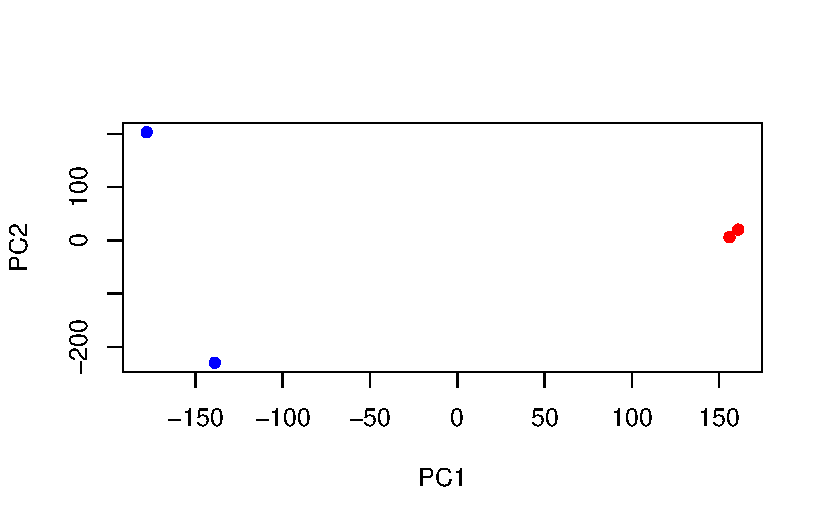
\includegraphics{class_16_files/figure-pdf/unnamed-chunk-8-1.pdf}

}

\end{figure}

\begin{quote}
Q. Use ggplot to make a similar figure of PC1 vs PC2 and a seperate
figure PC1 vs PC3 and PC2 vs PC3.
\end{quote}

\begin{Shaded}
\begin{Highlighting}[]
\FunctionTok{library}\NormalTok{(ggplot2)}
\FunctionTok{library}\NormalTok{(ggrepel)}

\CommentTok{\# Make metadata object for the samples}
\NormalTok{colData }\OtherTok{\textless{}{-}} \FunctionTok{data.frame}\NormalTok{(}\AttributeTok{condition =} \FunctionTok{factor}\NormalTok{(}\FunctionTok{rep}\NormalTok{(}\FunctionTok{c}\NormalTok{(}\StringTok{"control"}\NormalTok{, }\StringTok{"treatment"}\NormalTok{), }\AttributeTok{each =} \DecValTok{2}\NormalTok{)))}
\FunctionTok{rownames}\NormalTok{(colData) }\OtherTok{\textless{}{-}} \FunctionTok{colnames}\NormalTok{(txi.kallisto}\SpecialCharTok{$}\NormalTok{counts)}

\CommentTok{\# Make the data.frame for ggplot }
\NormalTok{y }\OtherTok{\textless{}{-}} \FunctionTok{as.data.frame}\NormalTok{(pca}\SpecialCharTok{$}\NormalTok{x)}
\NormalTok{y}\SpecialCharTok{$}\NormalTok{Condition }\OtherTok{\textless{}{-}} \FunctionTok{as.factor}\NormalTok{(colData}\SpecialCharTok{$}\NormalTok{condition)}

\FunctionTok{ggplot}\NormalTok{(y) }\SpecialCharTok{+}
  \FunctionTok{aes}\NormalTok{(PC1, PC2, }\AttributeTok{col=}\NormalTok{Condition) }\SpecialCharTok{+}
  \FunctionTok{geom\_point}\NormalTok{() }\SpecialCharTok{+}
  \FunctionTok{geom\_text\_repel}\NormalTok{(}\AttributeTok{label=}\FunctionTok{rownames}\NormalTok{(y)) }\SpecialCharTok{+}
  \FunctionTok{theme\_bw}\NormalTok{()}
\end{Highlighting}
\end{Shaded}

\begin{figure}[H]

{\centering 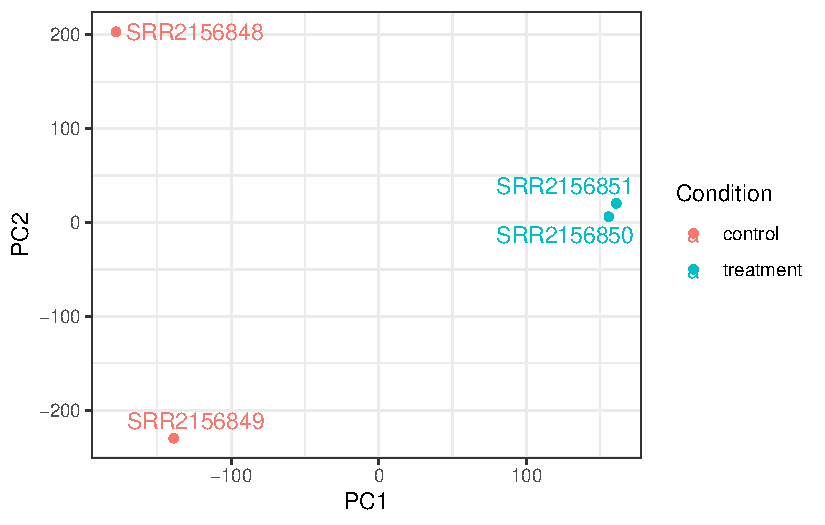
\includegraphics{class_16_files/figure-pdf/unnamed-chunk-9-1.pdf}

}

\end{figure}

\hypertarget{differential-expression-analysis}{%
\subsection{Differential-expression
analysis}\label{differential-expression-analysis}}

We can use DESeq2 to complete the differential-expression analysis that
we are already familiar with:

\begin{Shaded}
\begin{Highlighting}[]
\FunctionTok{library}\NormalTok{(DESeq2)}
\end{Highlighting}
\end{Shaded}

\begin{Shaded}
\begin{Highlighting}[]
\NormalTok{sampleTable }\OtherTok{\textless{}{-}} \FunctionTok{data.frame}\NormalTok{(}\AttributeTok{condition =} \FunctionTok{factor}\NormalTok{(}\FunctionTok{rep}\NormalTok{(}\FunctionTok{c}\NormalTok{(}\StringTok{"control"}\NormalTok{, }\StringTok{"treatment"}\NormalTok{), }\AttributeTok{each =} \DecValTok{2}\NormalTok{)))}
\FunctionTok{rownames}\NormalTok{(sampleTable) }\OtherTok{\textless{}{-}} \FunctionTok{colnames}\NormalTok{(txi.kallisto}\SpecialCharTok{$}\NormalTok{counts)}
\end{Highlighting}
\end{Shaded}

\begin{Shaded}
\begin{Highlighting}[]
\NormalTok{dds }\OtherTok{\textless{}{-}} \FunctionTok{DESeqDataSetFromTximport}\NormalTok{(txi.kallisto,}
\NormalTok{                                sampleTable, }
                                \SpecialCharTok{\textasciitilde{}}\NormalTok{condition)}
\end{Highlighting}
\end{Shaded}

\begin{verbatim}
using counts and average transcript lengths from tximport
\end{verbatim}

using counts and average transcript lengths from tximport

\begin{Shaded}
\begin{Highlighting}[]
\NormalTok{dds }\OtherTok{\textless{}{-}} \FunctionTok{DESeq}\NormalTok{(dds)}
\end{Highlighting}
\end{Shaded}

\begin{verbatim}
estimating size factors
\end{verbatim}

\begin{verbatim}
using 'avgTxLength' from assays(dds), correcting for library size
\end{verbatim}

\begin{verbatim}
estimating dispersions
\end{verbatim}

\begin{verbatim}
gene-wise dispersion estimates
\end{verbatim}

\begin{verbatim}
mean-dispersion relationship
\end{verbatim}

\begin{verbatim}
-- note: fitType='parametric', but the dispersion trend was not well captured by the
   function: y = a/x + b, and a local regression fit was automatically substituted.
   specify fitType='local' or 'mean' to avoid this message next time.
\end{verbatim}

\begin{verbatim}
final dispersion estimates
\end{verbatim}

\begin{verbatim}
fitting model and testing
\end{verbatim}

\begin{Shaded}
\begin{Highlighting}[]
\NormalTok{res }\OtherTok{\textless{}{-}} \FunctionTok{results}\NormalTok{(dds)}
\FunctionTok{head}\NormalTok{(res)}
\end{Highlighting}
\end{Shaded}

\begin{verbatim}
log2 fold change (MLE): condition treatment vs control 
Wald test p-value: condition treatment vs control 
DataFrame with 6 rows and 6 columns
                 baseMean log2FoldChange     lfcSE      stat    pvalue
                <numeric>      <numeric> <numeric> <numeric> <numeric>
ENST00000539570  0.000000             NA        NA        NA        NA
ENST00000576455  0.761453       3.155061   4.86052 0.6491203  0.516261
ENST00000510508  0.000000             NA        NA        NA        NA
ENST00000474471  0.484938       0.181923   4.24871 0.0428185  0.965846
ENST00000381700  0.000000             NA        NA        NA        NA
ENST00000445946  0.000000             NA        NA        NA        NA
                     padj
                <numeric>
ENST00000539570        NA
ENST00000576455        NA
ENST00000510508        NA
ENST00000474471        NA
ENST00000381700        NA
ENST00000445946        NA
\end{verbatim}

These results could go on to be visualized and subjected to pathway
analysis.



\end{document}
